\begin{figure}[htb]
%\centering
%\textbf{Living area for construction types of three typologies}\\
%\vspace{-1cm} 

%\hspace{-2.5cm}
  \begin{tabular}{p{0.43\linewidth} p{0.33\linewidth} p{0.43\linewidth}}
  %\begin{tabular}{lll}
\hspace{-2.5cm}
% Created by tikzDevice version 0.6.2-92-0ad2792 on 2013-10-13 23:40:46
% !TEX encoding = UTF-8 Unicode
\begin{tikzpicture}[x=1pt,y=1pt]
\definecolor[named]{fillColor}{rgb}{1.00,1.00,1.00}
\path[use as bounding box,fill=fillColor,fill opacity=0.00] (0,0) rectangle
 (216.81,216.81);
\begin{scope}
\path[clip] ( 49.20, 61.20) rectangle (191.61,167.61);
\definecolor[named]{drawColor}{rgb}{0.00,0.00,0.00}

\path[draw=drawColor,line width= 1.2pt,line join=round] ( 55.67, 65.53) -- ( 65.26, 65.53);

\path[draw=drawColor,line width= 0.4pt,dash pattern=on 4pt off 4pt ,line join=round,line cap=round] ( 60.47, 65.30) -- ( 60.47, 65.48);

\path[draw=drawColor,line width= 0.4pt,dash pattern=on 4pt off 4pt ,line join=round,line cap=round] ( 60.47, 65.63) -- ( 60.47, 65.63);

\path[draw=drawColor,line width= 0.4pt,line join=round,line cap=round] ( 58.07, 65.30) -- ( 62.87, 65.30);

\path[draw=drawColor,line width= 0.4pt,line join=round,line cap=round] ( 58.07, 65.63) -- ( 62.87, 65.63);

\path[draw=drawColor,line width= 0.4pt,line join=round,line cap=round] ( 55.67, 65.48) --
	( 65.26, 65.48) --
	( 65.26, 65.63) --
	( 55.67, 65.63) --
	( 55.67, 65.48);

\path[draw=drawColor,line width= 0.4pt,line join=round,line cap=round] ( 60.47, 65.95) circle (  2.25);

\path[draw=drawColor,line width= 0.4pt,line join=round,line cap=round] ( 60.47, 66.07) circle (  2.25);

\path[draw=drawColor,line width= 1.2pt,line join=round] ( 79.65, 76.14) -- ( 89.24, 76.14);

\path[draw=drawColor,line width= 0.4pt,dash pattern=on 4pt off 4pt ,line join=round,line cap=round] ( 84.44, 68.01) -- ( 84.44, 72.15);

\path[draw=drawColor,line width= 0.4pt,dash pattern=on 4pt off 4pt ,line join=round,line cap=round] ( 84.44, 81.33) -- ( 84.44, 76.14);

\path[draw=drawColor,line width= 0.4pt,line join=round,line cap=round] ( 82.05, 68.01) -- ( 86.84, 68.01);

\path[draw=drawColor,line width= 0.4pt,line join=round,line cap=round] ( 82.05, 81.33) -- ( 86.84, 81.33);

\path[draw=drawColor,line width= 0.4pt,line join=round,line cap=round] ( 79.65, 72.15) --
	( 89.24, 72.15) --
	( 89.24, 76.14) --
	( 79.65, 76.14) --
	( 79.65, 72.15);

\path[draw=drawColor,line width= 0.4pt,line join=round,line cap=round] ( 84.44, 84.15) circle (  2.25);

\path[draw=drawColor,line width= 1.2pt,line join=round] ( 91.64,142.79) -- (101.23,142.79);

\path[draw=drawColor,line width= 0.4pt,dash pattern=on 4pt off 4pt ,line join=round,line cap=round] ( 96.43,121.91) -- ( 96.43,121.91);

\path[draw=drawColor,line width= 0.4pt,dash pattern=on 4pt off 4pt ,line join=round,line cap=round] ( 96.43,163.67) -- ( 96.43,163.67);

\path[draw=drawColor,line width= 0.4pt,line join=round,line cap=round] ( 94.03,121.91) -- ( 98.83,121.91);

\path[draw=drawColor,line width= 0.4pt,line join=round,line cap=round] ( 94.03,163.67) -- ( 98.83,163.67);

\path[draw=drawColor,line width= 0.4pt,line join=round,line cap=round] ( 91.64,121.91) --
	(101.23,121.91) --
	(101.23,163.67) --
	( 91.64,163.67) --
	( 91.64,121.91);

\path[draw=drawColor,line width= 1.2pt,line join=round] (103.62, 68.01) -- (113.21, 68.01);

\path[draw=drawColor,line width= 0.4pt,dash pattern=on 4pt off 4pt ,line join=round,line cap=round] (108.42, 66.66) -- (108.42, 66.67);

\path[draw=drawColor,line width= 0.4pt,dash pattern=on 4pt off 4pt ,line join=round,line cap=round] (108.42, 72.98) -- (108.42, 71.68);

\path[draw=drawColor,line width= 0.4pt,line join=round,line cap=round] (106.02, 66.66) -- (110.82, 66.66);

\path[draw=drawColor,line width= 0.4pt,line join=round,line cap=round] (106.02, 72.98) -- (110.82, 72.98);

\path[draw=drawColor,line width= 0.4pt,line join=round,line cap=round] (103.62, 66.67) --
	(113.21, 66.67) --
	(113.21, 71.68) --
	(103.62, 71.68) --
	(103.62, 66.67);

\path[draw=drawColor,line width= 0.4pt,line join=round,line cap=round] (108.42, 80.37) circle (  2.25);

\path[draw=drawColor,line width= 1.2pt,line join=round] (175.55, 65.31) -- (185.14, 65.31);

\path[draw=drawColor,line width= 0.4pt,dash pattern=on 4pt off 4pt ,line join=round,line cap=round] (180.34, 65.14) -- (180.34, 65.28);

\path[draw=drawColor,line width= 0.4pt,dash pattern=on 4pt off 4pt ,line join=round,line cap=round] (180.34, 65.49) -- (180.34, 65.45);

\path[draw=drawColor,line width= 0.4pt,line join=round,line cap=round] (177.94, 65.14) -- (182.74, 65.14);

\path[draw=drawColor,line width= 0.4pt,line join=round,line cap=round] (177.94, 65.49) -- (182.74, 65.49);

\path[draw=drawColor,line width= 0.4pt,line join=round,line cap=round] (175.55, 65.28) --
	(185.14, 65.28) --
	(185.14, 65.45) --
	(175.55, 65.45) --
	(175.55, 65.28);
\end{scope}
\begin{scope}
\path[clip] (  0.00,  0.00) rectangle (216.81,216.81);
\definecolor[named]{drawColor}{rgb}{0.00,0.00,0.00}

\path[draw=drawColor,line width= 0.4pt,line join=round,line cap=round] ( 60.47, 61.20) -- (180.34, 61.20);

\path[draw=drawColor,line width= 0.4pt,line join=round,line cap=round] ( 60.47, 61.20) -- ( 60.47, 55.20);

\path[draw=drawColor,line width= 0.4pt,line join=round,line cap=round] ( 72.46, 61.20) -- ( 72.46, 55.20);

\path[draw=drawColor,line width= 0.4pt,line join=round,line cap=round] ( 84.44, 61.20) -- ( 84.44, 55.20);

\path[draw=drawColor,line width= 0.4pt,line join=round,line cap=round] ( 96.43, 61.20) -- ( 96.43, 55.20);

\path[draw=drawColor,line width= 0.4pt,line join=round,line cap=round] (108.42, 61.20) -- (108.42, 55.20);

\path[draw=drawColor,line width= 0.4pt,line join=round,line cap=round] (120.41, 61.20) -- (120.41, 55.20);

\path[draw=drawColor,line width= 0.4pt,line join=round,line cap=round] (132.39, 61.20) -- (132.39, 55.20);

\path[draw=drawColor,line width= 0.4pt,line join=round,line cap=round] (144.38, 61.20) -- (144.38, 55.20);

\path[draw=drawColor,line width= 0.4pt,line join=round,line cap=round] (156.37, 61.20) -- (156.37, 55.20);

\path[draw=drawColor,line width= 0.4pt,line join=round,line cap=round] (168.35, 61.20) -- (168.35, 55.20);

\path[draw=drawColor,line width= 0.4pt,line join=round,line cap=round] (180.34, 61.20) -- (180.34, 55.20);

% \node[text=drawColor,anchor=base,inner sep=0pt, outer sep=0pt, scale=  1.00] at ( 60.47, 39.60) {EFH};
% 
% \node[text=drawColor,anchor=base,inner sep=0pt, outer sep=0pt, scale=  1.00] at ( 96.43, 39.60) {HH};
% 
% \node[text=drawColor,anchor=base,inner sep=0pt, outer sep=0pt, scale=  1.00] at (132.39, 39.60) {MFH-E};
% 
% \node[text=drawColor,anchor=base,inner sep=0pt, outer sep=0pt, scale=  1.00] at (180.34, 39.60) {RDH};

\path[draw=drawColor,line width= 0.4pt,line join=round,line cap=round] ( 49.20, 64.75) -- ( 49.20,147.13);

\path[draw=drawColor,line width= 0.4pt,line join=round,line cap=round] ( 49.20, 64.75) -- ( 43.20, 64.75);

\path[draw=drawColor,line width= 0.4pt,line join=round,line cap=round] ( 49.20, 92.21) -- ( 43.20, 92.21);

\path[draw=drawColor,line width= 0.4pt,line join=round,line cap=round] ( 49.20,119.67) -- ( 43.20,119.67);

\path[draw=drawColor,line width= 0.4pt,line join=round,line cap=round] ( 49.20,147.13) -- ( 43.20,147.13);

\node[text=drawColor,rotate= 90.00,anchor=base,inner sep=0pt, outer sep=0pt, scale=  1.00] at ( 34.80, 64.75) {0};

\node[text=drawColor,rotate= 90.00,anchor=base,inner sep=0pt, outer sep=0pt, scale=  1.00] at ( 34.80, 92.21) {5000};

\node[text=drawColor,rotate= 90.00,anchor=base,inner sep=0pt, outer sep=0pt, scale=  1.00] at ( 34.80,147.13) {15000};

\node[text=drawColor,anchor=west, inner sep=0pt, outer sep=0pt, scale=  1.00]
at (49.20,180) {\textbf{(a) Blesl (table~\ref{tab:BW})}
\label{fig:AreaBleslA}
};

\path[draw=drawColor,line width= 0.4pt,line join=round,line cap=round] ( 49.20, 61.20) --
	(191.61, 61.20) --
	(191.61,167.61) --
	( 49.20,167.61) --
	( 49.20, 61.20);
\end{scope}
\begin{scope}
\path[clip] ( 49.20, 61.20) rectangle (191.61,167.61);
\definecolor[named]{drawColor}{rgb}{1.00,0.00,0.00}

\path[draw=drawColor,line width= 0.4pt,line join=round,line cap=round] ( 49.20, 86.71) -- (191.61, 86.78);
 
\path[draw=drawColor,line width= 0.4pt,line join=round,line cap=round] ( 49.20,119.67) -- (191.61,119.73);
\end{scope}
\end{tikzpicture}&
\hspace{-3.8cm}
% Created by tikzDevice version 0.6.2-92-0ad2792 on 2013-10-13 23:40:46
% !TEX encoding = UTF-8 Unicode
\begin{tikzpicture}[x=1pt,y=1pt]
\definecolor[named]{fillColor}{rgb}{1.00,1.00,1.00}
\path[use as bounding box,fill=fillColor,fill opacity=0.00] (0,0) rectangle (216.81,216.81);
\begin{scope}
\path[clip] ( 49.20, 61.20) rectangle (191.61,167.61);
\definecolor[named]{drawColor}{rgb}{0.00,0.00,0.00}

\path[draw=drawColor,line width= 1.2pt,line join=round] ( 55.67, 65.47) -- ( 65.26, 65.47);

\path[draw=drawColor,line width= 0.4pt,dash pattern=on 4pt off 4pt ,line join=round,line cap=round] ( 60.47, 65.22) -- ( 60.47, 65.37);

\path[draw=drawColor,line width= 0.4pt,dash pattern=on 4pt off 4pt ,line join=round,line cap=round] ( 60.47, 66.17) -- ( 60.47, 65.76);

\path[draw=drawColor,line width= 0.4pt,line join=round,line cap=round] ( 58.07, 65.22) -- ( 62.87, 65.22);

\path[draw=drawColor,line width= 0.4pt,line join=round,line cap=round] ( 58.07, 66.17) -- ( 62.87, 66.17);

\path[draw=drawColor,line width= 0.4pt,line join=round,line cap=round] ( 55.67, 65.37) --
	( 65.26, 65.37) --
	( 65.26, 65.76) --
	( 55.67, 65.76) --
	( 55.67, 65.37);

\path[draw=drawColor,line width= 1.2pt,line join=round] ( 79.65, 72.67) -- ( 89.24, 72.67);

\path[draw=drawColor,line width= 0.4pt,dash pattern=on 4pt off 4pt ,line join=round,line cap=round] ( 84.44, 68.81) -- ( 84.44, 72.08);

\path[draw=drawColor,line width= 0.4pt,dash pattern=on 4pt off 4pt ,line join=round,line cap=round] ( 84.44, 84.09) -- ( 84.44, 81.26);

\path[draw=drawColor,line width= 0.4pt,line join=round,line cap=round] ( 82.05, 68.81) -- ( 86.84, 68.81);

\path[draw=drawColor,line width= 0.4pt,line join=round,line cap=round] ( 82.05, 84.09) -- ( 86.84, 84.09);

\path[draw=drawColor,line width= 0.4pt,line join=round,line cap=round] ( 79.65, 72.08) --
	( 89.24, 72.08) --
	( 89.24, 81.26) --
	( 79.65, 81.26) --
	( 79.65, 72.08);

\path[draw=drawColor,line width= 1.2pt,line join=round] ( 91.64,142.77) -- (101.23,142.77);

\path[draw=drawColor,line width= 0.4pt,dash pattern=on 4pt off 4pt ,line join=round,line cap=round] ( 96.43,121.87) -- ( 96.43,121.87);

\path[draw=drawColor,line width= 0.4pt,dash pattern=on 4pt off 4pt ,line join=round,line cap=round] ( 96.43,163.67) -- ( 96.43,163.67);

\path[draw=drawColor,line width= 0.4pt,line join=round,line cap=round] ( 94.03,121.87) -- ( 98.83,121.87);

\path[draw=drawColor,line width= 0.4pt,line join=round,line cap=round] ( 94.03,163.67) -- ( 98.83,163.67);

\path[draw=drawColor,line width= 0.4pt,line join=round,line cap=round] ( 91.64,121.87) --
	(101.23,121.87) --
	(101.23,163.67) --
	( 91.64,163.67) --
	( 91.64,121.87);

\path[draw=drawColor,line width= 1.2pt,line join=round] (103.62, 67.99) -- (113.21, 67.99);

\path[draw=drawColor,line width= 0.4pt,dash pattern=on 4pt off 4pt ,line join=round,line cap=round] (108.42, 66.22) -- (108.42, 67.00);

\path[draw=drawColor,line width= 0.4pt,dash pattern=on 4pt off 4pt ,line join=round,line cap=round] (108.42, 68.83) -- (108.42, 68.83);

\path[draw=drawColor,line width= 0.4pt,line join=round,line cap=round] (106.02, 66.22) -- (110.82, 66.22);

\path[draw=drawColor,line width= 0.4pt,line join=round,line cap=round] (106.02, 68.83) -- (110.82, 68.83);

\path[draw=drawColor,line width= 0.4pt,line join=round,line cap=round] (103.62, 67.00) --
	(113.21, 67.00) --
	(113.21, 68.83) --
	(103.62, 68.83) --
	(103.62, 67.00);

\path[draw=drawColor,line width= 0.4pt,line join=round,line cap=round] (108.42, 80.30) circle (  2.25);

\path[draw=drawColor,line width= 0.4pt,line join=round,line cap=round] (108.42, 75.61) circle (  2.25);

\path[draw=drawColor,line width= 1.2pt,line join=round] (175.55, 65.25) -- (185.14, 65.25);

\path[draw=drawColor,line width= 0.4pt,dash pattern=on 4pt off 4pt ,line join=round,line cap=round] (180.34, 65.14) -- (180.34, 65.20);

\path[draw=drawColor,line width= 0.4pt,dash pattern=on 4pt off 4pt ,line join=round,line cap=round] (180.34, 65.42) -- (180.34, 65.41);

\path[draw=drawColor,line width= 0.4pt,line join=round,line cap=round] (177.94, 65.14) -- (182.74, 65.14);

\path[draw=drawColor,line width= 0.4pt,line join=round,line cap=round] (177.94, 65.42) -- (182.74, 65.42);

\path[draw=drawColor,line width= 0.4pt,line join=round,line cap=round] (175.55, 65.20) --
	(185.14, 65.20) --
	(185.14, 65.41) --
	(175.55, 65.41) --
	(175.55, 65.20);
\end{scope}
\begin{scope}
\path[clip] (  0.00,  0.00) rectangle (216.81,216.81);
\definecolor[named]{drawColor}{rgb}{0.00,0.00,0.00}

\path[draw=drawColor,line width= 0.4pt,line join=round,line cap=round] ( 60.47, 61.20) -- (180.34, 61.20);

\path[draw=drawColor,line width= 0.4pt,line join=round,line cap=round] ( 60.47, 61.20) -- ( 60.47, 55.20);

\path[draw=drawColor,line width= 0.4pt,line join=round,line cap=round] ( 72.46, 61.20) -- ( 72.46, 55.20);

\path[draw=drawColor,line width= 0.4pt,line join=round,line cap=round] ( 84.44, 61.20) -- ( 84.44, 55.20);

\path[draw=drawColor,line width= 0.4pt,line join=round,line cap=round] ( 96.43, 61.20) -- ( 96.43, 55.20);

\path[draw=drawColor,line width= 0.4pt,line join=round,line cap=round] (108.42, 61.20) -- (108.42, 55.20);

\path[draw=drawColor,line width= 0.4pt,line join=round,line cap=round] (120.41, 61.20) -- (120.41, 55.20);

\path[draw=drawColor,line width= 0.4pt,line join=round,line cap=round] (132.39, 61.20) -- (132.39, 55.20);

\path[draw=drawColor,line width= 0.4pt,line join=round,line cap=round] (144.38, 61.20) -- (144.38, 55.20);

\path[draw=drawColor,line width= 0.4pt,line join=round,line cap=round] (156.37, 61.20) -- (156.37, 55.20);

\path[draw=drawColor,line width= 0.4pt,line join=round,line cap=round] (168.35, 61.20) -- (168.35, 55.20);

\path[draw=drawColor,line width= 0.4pt,line join=round,line cap=round] (180.34, 61.20) -- (180.34, 55.20);

% \node[text=drawColor,anchor=base,inner sep=0pt, outer sep=0pt, scale=  1.00] at ( 60.47, 39.60) {EFH};
% 
% \node[text=drawColor,anchor=base,inner sep=0pt, outer sep=0pt, scale=  1.00] at ( 96.43, 39.60) {HH};
% 
% \node[text=drawColor,anchor=base,inner sep=0pt, outer sep=0pt, scale=  1.00] at (132.39, 39.60) {MFH-E};
% 
% \node[text=drawColor,anchor=base,inner sep=0pt, outer sep=0pt, scale=  1.00] at (180.34, 39.60) {RDH};

\path[draw=drawColor,line width= 0.4pt,line join=round,line cap=round] ( 49.20, 64.66) -- ( 49.20,147.11);

\path[draw=drawColor,line width= 0.4pt,line join=round,line cap=round] ( 49.20, 64.66) -- ( 43.20, 64.66);

\path[draw=drawColor,line width= 0.4pt,line join=round,line cap=round] ( 49.20, 92.15) -- ( 43.20, 92.15);

\path[draw=drawColor,line width= 0.4pt,line join=round,line cap=round] ( 49.20,119.63) -- ( 43.20,119.63);

\path[draw=drawColor,line width= 0.4pt,line join=round,line cap=round] ( 49.20,147.11) -- ( 43.20,147.11);

% \node[text=drawColor,rotate= 90.00,anchor=base,inner sep=0pt, outer sep=0pt, scale=  1.00] at ( 34.80, 64.66) {0};
% 
% \node[text=drawColor,rotate= 90.00,anchor=base,inner sep=0pt, outer sep=0pt, scale=  1.00] at ( 34.80, 92.15) {5000};
% 
% \node[text=drawColor,rotate= 90.00,anchor=base,inner sep=0pt, outer sep=0pt, scale=  1.00] at ( 34.80,147.11) {15000};

\node[text=drawColor,anchor=west, inner sep=0pt, outer sep=0pt, scale=  1.00]
at (49.20,180) {\textbf{(b) IWU-de
(table~\ref{tab:IWU-de})}
\label{fig:AreaIWUdeA}
};

\path[draw=drawColor,line width= 0.4pt,line join=round,line cap=round] ( 49.20, 61.20) --
	(191.61, 61.20) --
	(191.61,167.61) --
	( 49.20,167.61) --
	( 49.20, 61.20);
\end{scope}
\begin{scope}
\path[clip] ( 49.20, 61.20) rectangle (191.61,167.61);
\definecolor[named]{drawColor}{rgb}{1.00,0.00,0.00}

\path[draw=drawColor,line width= 0.4pt,line join=round,line cap=round] ( 49.20, 86.65) -- (191.61, 86.71);

\path[draw=drawColor,line width= 0.4pt,line join=round,line cap=round] ( 49.20,119.63) -- (191.61,119.69);
\end{scope}
\end{tikzpicture}
&
\hspace{-3.8cm}
% Created by tikzDevice version 0.6.2-92-0ad2792 on 2013-10-13 23:40:46
% !TEX encoding = UTF-8 Unicode
\begin{tikzpicture}[x=1pt,y=1pt]
\definecolor[named]{fillColor}{rgb}{1.00,1.00,1.00}
\path[use as bounding box,fill=fillColor,fill opacity=0.00] (0,0) rectangle (216.81,216.81);
\begin{scope}
\path[clip] ( 49.20, 61.20) rectangle (191.61,167.61);
\definecolor[named]{drawColor}{rgb}{0.00,0.00,0.00}

\path[draw=drawColor,line width= 1.2pt,line join=round] ( 55.67, 65.59) -- ( 65.26, 65.59);

\path[draw=drawColor,line width= 0.4pt,dash pattern=on 4pt off 4pt ,line join=round,line cap=round] ( 60.47, 65.22) -- ( 60.47, 65.39);

\path[draw=drawColor,line width= 0.4pt,dash pattern=on 4pt off 4pt ,line join=round,line cap=round] ( 60.47, 66.17) -- ( 60.47, 65.87);

\path[draw=drawColor,line width= 0.4pt,line join=round,line cap=round] ( 58.07, 65.22) -- ( 62.87, 65.22);

\path[draw=drawColor,line width= 0.4pt,line join=round,line cap=round] ( 58.07, 66.17) -- ( 62.87, 66.17);

\path[draw=drawColor,line width= 0.4pt,line join=round,line cap=round] ( 55.67, 65.39) --
	( 65.26, 65.39) --
	( 65.26, 65.87) --
	( 55.67, 65.87) --
	( 55.67, 65.39);

\path[draw=drawColor,line width= 1.2pt,line join=round] ( 67.66, 65.64) -- ( 77.25, 65.64);

\path[draw=drawColor,line width= 0.4pt,dash pattern=on 4pt off 4pt ,line join=round,line cap=round] ( 72.46, 65.53) -- ( 72.46, 65.53);

\path[draw=drawColor,line width= 0.4pt,dash pattern=on 4pt off 4pt ,line join=round,line cap=round] ( 72.46, 65.76) -- ( 72.46, 65.76);

\path[draw=drawColor,line width= 0.4pt,line join=round,line cap=round] ( 70.06, 65.53) -- ( 74.85, 65.53);

\path[draw=drawColor,line width= 0.4pt,line join=round,line cap=round] ( 70.06, 65.76) -- ( 74.85, 65.76);

\path[draw=drawColor,line width= 0.4pt,line join=round,line cap=round] ( 67.66, 65.53) --
	( 77.25, 65.53) --
	( 77.25, 65.76) --
	( 67.66, 65.76) --
	( 67.66, 65.53);

\path[draw=drawColor,line width= 1.2pt,line join=round] ( 79.65, 72.67) -- ( 89.24, 72.67);

\path[draw=drawColor,line width= 0.4pt,dash pattern=on 4pt off 4pt ,line join=round,line cap=round] ( 84.44, 68.81) -- ( 84.44, 72.08);

\path[draw=drawColor,line width= 0.4pt,dash pattern=on 4pt off 4pt ,line join=round,line cap=round] ( 84.44, 84.09) -- ( 84.44, 81.26);

\path[draw=drawColor,line width= 0.4pt,line join=round,line cap=round] ( 82.05, 68.81) -- ( 86.84, 68.81);

\path[draw=drawColor,line width= 0.4pt,line join=round,line cap=round] ( 82.05, 84.09) -- ( 86.84, 84.09);

\path[draw=drawColor,line width= 0.4pt,line join=round,line cap=round] ( 79.65, 72.08) --
	( 89.24, 72.08) --
	( 89.24, 81.26) --
	( 79.65, 81.26) --
	( 79.65, 72.08);

\path[draw=drawColor,line width= 1.2pt,line join=round] ( 91.64,142.77) -- (101.23,142.77);

\path[draw=drawColor,line width= 0.4pt,dash pattern=on 4pt off 4pt ,line join=round,line cap=round] ( 96.43,121.87) -- ( 96.43,121.87);

\path[draw=drawColor,line width= 0.4pt,dash pattern=on 4pt off 4pt ,line join=round,line cap=round] ( 96.43,163.67) -- ( 96.43,163.67);

\path[draw=drawColor,line width= 0.4pt,line join=round,line cap=round] ( 94.03,121.87) -- ( 98.83,121.87);

\path[draw=drawColor,line width= 0.4pt,line join=round,line cap=round] ( 94.03,163.67) -- ( 98.83,163.67);

\path[draw=drawColor,line width= 0.4pt,line join=round,line cap=round] ( 91.64,121.87) --
	(101.23,121.87) --
	(101.23,163.67) --
	( 91.64,163.67) --
	( 91.64,121.87);

\path[draw=drawColor,line width= 1.2pt,line join=round] (103.62, 67.93) -- (113.21, 67.93);

\path[draw=drawColor,line width= 0.4pt,dash pattern=on 4pt off 4pt ,line join=round,line cap=round] (108.42, 66.59) -- (108.42, 67.41);

\path[draw=drawColor,line width= 0.4pt,dash pattern=on 4pt off 4pt ,line join=round,line cap=round] (108.42, 68.55) -- (108.42, 68.30);

\path[draw=drawColor,line width= 0.4pt,line join=round,line cap=round] (106.02, 66.59) -- (110.82, 66.59);

\path[draw=drawColor,line width= 0.4pt,line join=round,line cap=round] (106.02, 68.55) -- (110.82, 68.55);

\path[draw=drawColor,line width= 0.4pt,line join=round,line cap=round] (103.62, 67.41) --
	(113.21, 67.41) --
	(113.21, 68.30) --
	(103.62, 68.30) --
	(103.62, 67.41);

\path[draw=drawColor,line width= 0.4pt,line join=round,line cap=round] (108.42, 80.30) circle (  2.25);

\path[draw=drawColor,line width= 1.2pt,line join=round] (115.61, 66.22) -- (125.20, 66.22);

\path[draw=drawColor,line width= 0.4pt,dash pattern=on 4pt off 4pt ,line join=round,line cap=round] (120.41, 66.22) -- (120.41, 66.22);

\path[draw=drawColor,line width= 0.4pt,dash pattern=on 4pt off 4pt ,line join=round,line cap=round] (120.41, 66.22) -- (120.41, 66.22);

\path[draw=drawColor,line width= 0.4pt,line join=round,line cap=round] (118.01, 66.22) -- (122.80, 66.22);

\path[draw=drawColor,line width= 0.4pt,line join=round,line cap=round] (118.01, 66.22) -- (122.80, 66.22);

\path[draw=drawColor,line width= 0.4pt,line join=round,line cap=round] (115.61, 66.22) --
	(125.20, 66.22) --
	(125.20, 66.22) --
	(115.61, 66.22) --
	(115.61, 66.22);

\path[draw=drawColor,line width= 1.2pt,line join=round] (175.55, 65.23) -- (185.14, 65.23);

\path[draw=drawColor,line width= 0.4pt,dash pattern=on 4pt off 4pt ,line join=round,line cap=round] (180.34, 65.14) -- (180.34, 65.20);

\path[draw=drawColor,line width= 0.4pt,dash pattern=on 4pt off 4pt ,line join=round,line cap=round] (180.34, 65.30) -- (180.34, 65.28);

\path[draw=drawColor,line width= 0.4pt,line join=round,line cap=round] (177.94, 65.14) -- (182.74, 65.14);

\path[draw=drawColor,line width= 0.4pt,line join=round,line cap=round] (177.94, 65.30) -- (182.74, 65.30);

\path[draw=drawColor,line width= 0.4pt,line join=round,line cap=round] (175.55, 65.20) --
	(185.14, 65.20) --
	(185.14, 65.28) --
	(175.55, 65.28) --
	(175.55, 65.20);

\path[draw=drawColor,line width= 0.4pt,line join=round,line cap=round] (180.34, 65.41) circle (  2.25);
\end{scope}
\begin{scope}
\path[clip] (  0.00,  0.00) rectangle (216.81,216.81);
\definecolor[named]{drawColor}{rgb}{0.00,0.00,0.00}

\path[draw=drawColor,line width= 0.4pt,line join=round,line cap=round] ( 60.47, 61.20) -- (180.34, 61.20);

\path[draw=drawColor,line width= 0.4pt,line join=round,line cap=round] ( 60.47, 61.20) -- ( 60.47, 55.20);

\path[draw=drawColor,line width= 0.4pt,line join=round,line cap=round] ( 72.46, 61.20) -- ( 72.46, 55.20);

\path[draw=drawColor,line width= 0.4pt,line join=round,line cap=round] ( 84.44, 61.20) -- ( 84.44, 55.20);

\path[draw=drawColor,line width= 0.4pt,line join=round,line cap=round] ( 96.43, 61.20) -- ( 96.43, 55.20);

\path[draw=drawColor,line width= 0.4pt,line join=round,line cap=round] (108.42, 61.20) -- (108.42, 55.20);

\path[draw=drawColor,line width= 0.4pt,line join=round,line cap=round] (120.41, 61.20) -- (120.41, 55.20);

\path[draw=drawColor,line width= 0.4pt,line join=round,line cap=round] (132.39, 61.20) -- (132.39, 55.20);

\path[draw=drawColor,line width= 0.4pt,line join=round,line cap=round] (144.38, 61.20) -- (144.38, 55.20);

\path[draw=drawColor,line width= 0.4pt,line join=round,line cap=round] (156.37, 61.20) -- (156.37, 55.20);

\path[draw=drawColor,line width= 0.4pt,line join=round,line cap=round] (168.35, 61.20) -- (168.35, 55.20);

\path[draw=drawColor,line width= 0.4pt,line join=round,line cap=round] (180.34, 61.20) -- (180.34, 55.20);

% \node[text=drawColor,anchor=base,inner sep=0pt, outer sep=0pt, scale=  1.00] at ( 60.47, 39.60) {EFH};
% 
% \node[text=drawColor,anchor=base,inner sep=0pt, outer sep=0pt, scale=  1.00] at ( 96.43, 39.60) {HH};
% 
% \node[text=drawColor,anchor=base,inner sep=0pt, outer sep=0pt, scale=  1.00] at (132.39, 39.60) {MFH-E};
% 
% \node[text=drawColor,anchor=base,inner sep=0pt, outer sep=0pt, scale=  1.00] at (180.34, 39.60) {RDH};

\path[draw=drawColor,line width= 0.4pt,line join=round,line cap=round] ( 49.20, 64.66) -- ( 49.20,147.11);

\path[draw=drawColor,line width= 0.4pt,line join=round,line cap=round] ( 49.20, 64.66) -- ( 43.20, 64.66);

\path[draw=drawColor,line width= 0.4pt,line join=round,line cap=round] ( 49.20, 92.15) -- ( 43.20, 92.15);

\path[draw=drawColor,line width= 0.4pt,line join=round,line cap=round] ( 49.20,119.63) -- ( 43.20,119.63);

\path[draw=drawColor,line width= 0.4pt,line join=round,line cap=round] ( 49.20,147.11) -- ( 43.20,147.11);

% \node[text=drawColor,rotate= 90.00,anchor=base,inner sep=0pt, outer sep=0pt, scale=  1.00] at ( 34.80, 64.66) {0};
% 
% \node[text=drawColor,rotate= 90.00,anchor=base,inner sep=0pt, outer sep=0pt, scale=  1.00] at ( 34.80, 92.15) {5000};
% 
% \node[text=drawColor,rotate= 90.00,anchor=base,inner sep=0pt, outer sep=0pt, scale=  1.00] at ( 34.80,147.11) {15000};

\node[text=drawColor,anchor=west, inner sep=0pt, outer sep=0pt, scale=  1.00]
at (49.20,180) {\textbf{(c) IWU-he
(table~\ref{tab:IWU-he})}
\label{fig:AreaIWUheA}
};

\path[draw=drawColor,line width= 0.4pt,line join=round,line cap=round] ( 49.20, 61.20) --
	(191.61, 61.20) --
	(191.61,167.61) --
	( 49.20,167.61) --
	( 49.20, 61.20);
\end{scope}
\begin{scope}
\path[clip] ( 49.20, 61.20) rectangle (191.61,167.61);
\definecolor[named]{drawColor}{rgb}{1.00,0.00,0.00}

\path[draw=drawColor,line width= 0.4pt,line join=round,line cap=round] ( 49.20, 86.65) -- (191.61, 86.72);

\path[draw=drawColor,line width= 0.4pt,line join=round,line cap=round] ( 49.20,119.63) -- (191.61,119.70);
\end{scope}
<<<<<<< HEAD
\end{tikzpicture}
=======
\end{tikzpicture}
>>>>>>> 36a956db0f2ffb15b4b8091da9293464a1b25a0c
\\

%\vspace{-3cm} 
\hspace{-2.5cm}
% Created by tikzDevice version 0.6.2-92-0ad2792 on 2013-10-13 23:59:58
% !TEX encoding = UTF-8 Unicode
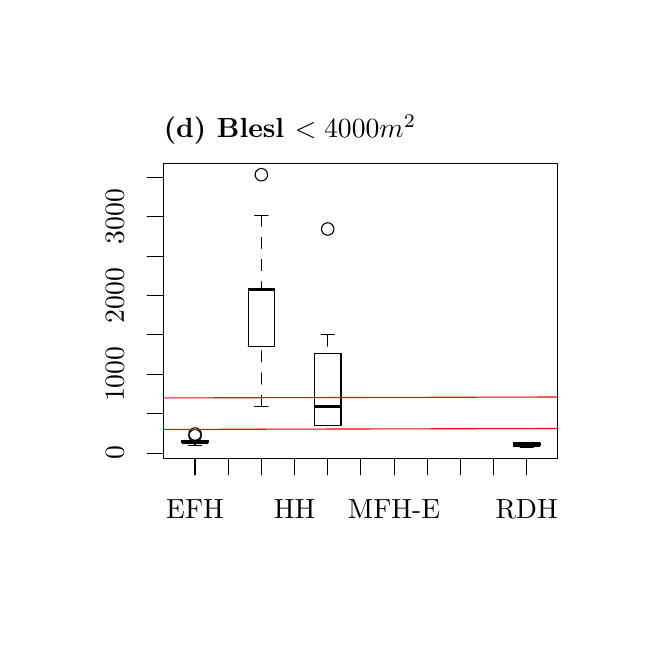
\begin{tikzpicture}[x=1pt,y=1pt]
\definecolor[named]{fillColor}{rgb}{1.00,1.00,1.00}
\path[use as bounding box,fill=fillColor,fill opacity=0.00] (0,0) rectangle (216.81,216.81);
\begin{scope}
\path[clip] ( 49.20, 61.20) rectangle (191.61,167.61);
\definecolor[named]{drawColor}{rgb}{0.00,0.00,0.00}

\path[draw=drawColor,line width= 1.2pt,line join=round] ( 55.67, 67.13) -- ( 65.26, 67.13);

\path[draw=drawColor,line width= 0.4pt,dash pattern=on 4pt off 4pt ,line join=round,line cap=round] ( 60.47, 65.97) -- ( 60.47, 66.91);

\path[draw=drawColor,line width= 0.4pt,dash pattern=on 4pt off 4pt ,line join=round,line cap=round] ( 60.47, 67.67) -- ( 60.47, 67.67);

\path[draw=drawColor,line width= 0.4pt,line join=round,line cap=round] ( 58.07, 65.97) -- ( 62.87, 65.97);

\path[draw=drawColor,line width= 0.4pt,line join=round,line cap=round] ( 58.07, 67.67) -- ( 62.87, 67.67);

\path[draw=drawColor,line width= 0.4pt,line join=round,line cap=round] ( 55.67, 66.91) --
	( 65.26, 66.91) --
	( 65.26, 67.67) --
	( 55.67, 67.67) --
	( 55.67, 66.91);

\path[draw=drawColor,line width= 0.4pt,line join=round,line cap=round] ( 60.47, 69.35) circle (  2.25);

\path[draw=drawColor,line width= 0.4pt,line join=round,line cap=round] ( 60.47, 69.98) circle (  2.25);

\path[draw=drawColor,line width= 1.2pt,line join=round] ( 79.65,122.15) -- ( 89.24,122.15);

\path[draw=drawColor,line width= 0.4pt,dash pattern=on 4pt off 4pt ,line join=round,line cap=round] ( 84.44, 80.03) -- ( 84.44,101.48);

\path[draw=drawColor,line width= 0.4pt,dash pattern=on 4pt off 4pt ,line join=round,line cap=round] ( 84.44,149.04) -- ( 84.44,122.15);

\path[draw=drawColor,line width= 0.4pt,line join=round,line cap=round] ( 82.05, 80.03) -- ( 86.84, 80.03);

\path[draw=drawColor,line width= 0.4pt,line join=round,line cap=round] ( 82.05,149.04) -- ( 86.84,149.04);

\path[draw=drawColor,line width= 0.4pt,line join=round,line cap=round] ( 79.65,101.48) --
	( 89.24,101.48) --
	( 89.24,122.15) --
	( 79.65,122.15) --
	( 79.65,101.48);

\path[draw=drawColor,line width= 0.4pt,line join=round,line cap=round] ( 84.44,163.67) circle (  2.25);

\path[draw=drawColor,line width= 1.2pt,line join=round] (103.62, 80.03) -- (113.21, 80.03);

\path[draw=drawColor,line width= 0.4pt,dash pattern=on 4pt off 4pt ,line join=round,line cap=round] (108.42, 73.02) -- (108.42, 73.08);

\path[draw=drawColor,line width= 0.4pt,dash pattern=on 4pt off 4pt ,line join=round,line cap=round] (108.42,105.78) -- (108.42, 99.04);

\path[draw=drawColor,line width= 0.4pt,line join=round,line cap=round] (106.02, 73.02) -- (110.82, 73.02);

\path[draw=drawColor,line width= 0.4pt,line join=round,line cap=round] (106.02,105.78) -- (110.82,105.78);

\path[draw=drawColor,line width= 0.4pt,line join=round,line cap=round] (103.62, 73.08) --
	(113.21, 73.08) --
	(113.21, 99.04) --
	(103.62, 99.04) --
	(103.62, 73.08);

\path[draw=drawColor,line width= 0.4pt,line join=round,line cap=round] (108.42,144.06) circle (  2.25);

\path[draw=drawColor,line width= 1.2pt,line join=round] (175.55, 66.02) -- (185.14, 66.02);

\path[draw=drawColor,line width= 0.4pt,dash pattern=on 4pt off 4pt ,line join=round,line cap=round] (180.34, 65.14) -- (180.34, 65.85);

\path[draw=drawColor,line width= 0.4pt,dash pattern=on 4pt off 4pt ,line join=round,line cap=round] (180.34, 66.96) -- (180.34, 66.73);

\path[draw=drawColor,line width= 0.4pt,line join=round,line cap=round] (177.94, 65.14) -- (182.74, 65.14);

\path[draw=drawColor,line width= 0.4pt,line join=round,line cap=round] (177.94, 66.96) -- (182.74, 66.96);

\path[draw=drawColor,line width= 0.4pt,line join=round,line cap=round] (175.55, 65.85) --
	(185.14, 65.85) --
	(185.14, 66.73) --
	(175.55, 66.73) --
	(175.55, 65.85);
\end{scope}
\begin{scope}
\path[clip] (  0.00,  0.00) rectangle (216.81,216.81);
\definecolor[named]{drawColor}{rgb}{0.00,0.00,0.00}

\path[draw=drawColor,line width= 0.4pt,line join=round,line cap=round] ( 60.47, 61.20) -- (180.34, 61.20);

\path[draw=drawColor,line width= 0.4pt,line join=round,line cap=round] ( 60.47, 61.20) -- ( 60.47, 55.20);

\path[draw=drawColor,line width= 0.4pt,line join=round,line cap=round] ( 72.46, 61.20) -- ( 72.46, 55.20);

\path[draw=drawColor,line width= 0.4pt,line join=round,line cap=round] ( 84.44, 61.20) -- ( 84.44, 55.20);

\path[draw=drawColor,line width= 0.4pt,line join=round,line cap=round] ( 96.43, 61.20) -- ( 96.43, 55.20);

\path[draw=drawColor,line width= 0.4pt,line join=round,line cap=round] (108.42, 61.20) -- (108.42, 55.20);

\path[draw=drawColor,line width= 0.4pt,line join=round,line cap=round] (120.41, 61.20) -- (120.41, 55.20);

\path[draw=drawColor,line width= 0.4pt,line join=round,line cap=round] (132.39, 61.20) -- (132.39, 55.20);

\path[draw=drawColor,line width= 0.4pt,line join=round,line cap=round] (144.38, 61.20) -- (144.38, 55.20);

\path[draw=drawColor,line width= 0.4pt,line join=round,line cap=round] (156.37, 61.20) -- (156.37, 55.20);

\path[draw=drawColor,line width= 0.4pt,line join=round,line cap=round] (168.35, 61.20) -- (168.35, 55.20);

\path[draw=drawColor,line width= 0.4pt,line join=round,line cap=round] (180.34, 61.20) -- (180.34, 55.20);

\node[text=drawColor,anchor=base,inner sep=0pt, outer sep=0pt, scale=  1.00] at ( 60.47, 39.60) {EFH};

\node[text=drawColor,anchor=base,inner sep=0pt, outer sep=0pt, scale=  1.00] at ( 96.43, 39.60) {HH};

\node[text=drawColor,anchor=base,inner sep=0pt, outer sep=0pt, scale=  1.00] at (132.39, 39.60) {MFH-E};

\node[text=drawColor,anchor=base,inner sep=0pt, outer sep=0pt, scale=  1.00] at (180.34, 39.60) {RDH};

\path[draw=drawColor,line width= 0.4pt,line join=round,line cap=round] ( 49.20, 63.09) -- ( 49.20,162.70);

\path[draw=drawColor,line width= 0.4pt,line join=round,line cap=round] ( 49.20, 63.09) -- ( 43.20, 63.09);

\path[draw=drawColor,line width= 0.4pt,line join=round,line cap=round] ( 49.20, 77.32) -- ( 43.20, 77.32);

\path[draw=drawColor,line width= 0.4pt,line join=round,line cap=round] ( 49.20, 91.55) -- ( 43.20, 91.55);

\path[draw=drawColor,line width= 0.4pt,line join=round,line cap=round] ( 49.20,105.78) -- ( 43.20,105.78);

\path[draw=drawColor,line width= 0.4pt,line join=round,line cap=round] ( 49.20,120.01) -- ( 43.20,120.01);

\path[draw=drawColor,line width= 0.4pt,line join=round,line cap=round] ( 49.20,134.24) -- ( 43.20,134.24);

\path[draw=drawColor,line width= 0.4pt,line join=round,line cap=round] ( 49.20,148.47) -- ( 43.20,148.47);

\path[draw=drawColor,line width= 0.4pt,line join=round,line cap=round] ( 49.20,162.70) -- ( 43.20,162.70);

\node[text=drawColor,rotate= 90.00,anchor=base,inner sep=0pt, outer sep=0pt, scale=  1.00] at ( 34.80, 63.09) {0};

\node[text=drawColor,rotate= 90.00,anchor=base,inner sep=0pt, outer sep=0pt, scale=  1.00] at ( 34.80, 91.55) {1000};

\node[text=drawColor,rotate= 90.00,anchor=base,inner sep=0pt, outer sep=0pt, scale=  1.00] at ( 34.80,120.01) {2000};

\node[text=drawColor,rotate= 90.00,anchor=base,inner sep=0pt, outer sep=0pt, scale=  1.00] at ( 34.80,148.47) {3000};

\node[text=drawColor,anchor=west, inner sep=0pt, outer sep=0pt, scale=  1.00]
at (49.20,180) {\textbf{(d) Blesl $< 4000 m^2$}
\label{fig:AreaBleslB}
};

\path[draw=drawColor,line width= 0.4pt,line join=round,line cap=round] ( 49.20, 61.20) --
	(191.61, 61.20) --
	(191.61,167.61) --
	( 49.20,167.61) --
	( 49.20, 61.20);
\end{scope}
\begin{scope}
\path[clip] ( 49.20, 61.20) rectangle (191.61,167.61);
\definecolor[named]{drawColor}{rgb}{1.00,0.00,0.00}

\path[draw=drawColor,line width= 0.4pt,line join=round,line cap=round] ( 49.20, 71.63) -- (191.61, 71.97);

\path[draw=drawColor,line width= 0.4pt,line join=round,line cap=round] ( 49.20, 83.02) -- (191.61, 83.35);
\end{scope}
\end{tikzpicture}&
%\vspace{-3cm} 
\hspace{-3.8cm}
% Created by tikzDevice version 0.6.2-92-0ad2792 on 2013-10-13 23:59:58
% !TEX encoding = UTF-8 Unicode
\begin{tikzpicture}[x=1pt,y=1pt]
\definecolor[named]{fillColor}{rgb}{1.00,1.00,1.00}
\path[use as bounding box,fill=fillColor,fill opacity=0.00] (0,0) rectangle (216.81,216.81);
\begin{scope}
\path[clip] ( 49.20, 61.20) rectangle (191.61,167.61);
\definecolor[named]{drawColor}{rgb}{0.00,0.00,0.00}

\path[draw=drawColor,line width= 1.2pt,line join=round] ( 55.67, 66.85) -- ( 65.26, 66.85);

\path[draw=drawColor,line width= 0.4pt,dash pattern=on 4pt off 4pt ,line join=round,line cap=round] ( 60.47, 65.54) -- ( 60.47, 66.33);

\path[draw=drawColor,line width= 0.4pt,dash pattern=on 4pt off 4pt ,line join=round,line cap=round] ( 60.47, 70.51) -- ( 60.47, 68.34);

\path[draw=drawColor,line width= 0.4pt,line join=round,line cap=round] ( 58.07, 65.54) -- ( 62.87, 65.54);

\path[draw=drawColor,line width= 0.4pt,line join=round,line cap=round] ( 58.07, 70.51) -- ( 62.87, 70.51);

\path[draw=drawColor,line width= 0.4pt,line join=round,line cap=round] ( 55.67, 66.33) --
	( 65.26, 66.33) --
	( 65.26, 68.34) --
	( 55.67, 68.34) --
	( 55.67, 66.33);

\path[draw=drawColor,line width= 1.2pt,line join=round] ( 79.65,104.30) -- ( 89.24,104.30);

\path[draw=drawColor,line width= 0.4pt,dash pattern=on 4pt off 4pt ,line join=round,line cap=round] ( 84.44, 84.20) -- ( 84.44,101.21);

\path[draw=drawColor,line width= 0.4pt,dash pattern=on 4pt off 4pt ,line join=round,line cap=round] ( 84.44,163.67) -- ( 84.44,148.98);

\path[draw=drawColor,line width= 0.4pt,line join=round,line cap=round] ( 82.05, 84.20) -- ( 86.84, 84.20);

\path[draw=drawColor,line width= 0.4pt,line join=round,line cap=round] ( 82.05,163.67) -- ( 86.84,163.67);

\path[draw=drawColor,line width= 0.4pt,line join=round,line cap=round] ( 79.65,101.21) --
	( 89.24,101.21) --
	( 89.24,148.98) --
	( 79.65,148.98) --
	( 79.65,101.21);

\path[draw=drawColor,line width= 1.2pt,line join=round] (103.62, 79.95) -- (113.21, 79.95);

\path[draw=drawColor,line width= 0.4pt,dash pattern=on 4pt off 4pt ,line join=round,line cap=round] (108.42, 70.77) -- (108.42, 74.83);

\path[draw=drawColor,line width= 0.4pt,dash pattern=on 4pt off 4pt ,line join=round,line cap=round] (108.42, 84.34) -- (108.42, 84.34);

\path[draw=drawColor,line width= 0.4pt,line join=round,line cap=round] (106.02, 70.77) -- (110.82, 70.77);

\path[draw=drawColor,line width= 0.4pt,line join=round,line cap=round] (106.02, 84.34) -- (110.82, 84.34);

\path[draw=drawColor,line width= 0.4pt,line join=round,line cap=round] (103.62, 74.83) --
	(113.21, 74.83) --
	(113.21, 84.34) --
	(103.62, 84.34) --
	(103.62, 74.83);

\path[draw=drawColor,line width= 0.4pt,line join=round,line cap=round] (108.42,143.96) circle (  2.25);

\path[draw=drawColor,line width= 0.4pt,line join=round,line cap=round] (108.42,119.56) circle (  2.25);

\path[draw=drawColor,line width= 1.2pt,line join=round] (175.55, 65.70) -- (185.14, 65.70);

\path[draw=drawColor,line width= 0.4pt,dash pattern=on 4pt off 4pt ,line join=round,line cap=round] (180.34, 65.14) -- (180.34, 65.46);

\path[draw=drawColor,line width= 0.4pt,dash pattern=on 4pt off 4pt ,line join=round,line cap=round] (180.34, 66.60) -- (180.34, 66.52);

\path[draw=drawColor,line width= 0.4pt,line join=round,line cap=round] (177.94, 65.14) -- (182.74, 65.14);

\path[draw=drawColor,line width= 0.4pt,line join=round,line cap=round] (177.94, 66.60) -- (182.74, 66.60);

\path[draw=drawColor,line width= 0.4pt,line join=round,line cap=round] (175.55, 65.46) --
	(185.14, 65.46) --
	(185.14, 66.52) --
	(175.55, 66.52) --
	(175.55, 65.46);
\end{scope}
\begin{scope}
\path[clip] (  0.00,  0.00) rectangle (216.81,216.81);
\definecolor[named]{drawColor}{rgb}{0.00,0.00,0.00}

\path[draw=drawColor,line width= 0.4pt,line join=round,line cap=round] ( 60.47, 61.20) -- (180.34, 61.20);

\path[draw=drawColor,line width= 0.4pt,line join=round,line cap=round] ( 60.47, 61.20) -- ( 60.47, 55.20);

\path[draw=drawColor,line width= 0.4pt,line join=round,line cap=round] ( 72.46, 61.20) -- ( 72.46, 55.20);

\path[draw=drawColor,line width= 0.4pt,line join=round,line cap=round] ( 84.44, 61.20) -- ( 84.44, 55.20);

\path[draw=drawColor,line width= 0.4pt,line join=round,line cap=round] ( 96.43, 61.20) -- ( 96.43, 55.20);

\path[draw=drawColor,line width= 0.4pt,line join=round,line cap=round] (108.42, 61.20) -- (108.42, 55.20);

\path[draw=drawColor,line width= 0.4pt,line join=round,line cap=round] (120.41, 61.20) -- (120.41, 55.20);

\path[draw=drawColor,line width= 0.4pt,line join=round,line cap=round] (132.39, 61.20) -- (132.39, 55.20);

\path[draw=drawColor,line width= 0.4pt,line join=round,line cap=round] (144.38, 61.20) -- (144.38, 55.20);

\path[draw=drawColor,line width= 0.4pt,line join=round,line cap=round] (156.37, 61.20) -- (156.37, 55.20);

\path[draw=drawColor,line width= 0.4pt,line join=round,line cap=round] (168.35, 61.20) -- (168.35, 55.20);

\path[draw=drawColor,line width= 0.4pt,line join=round,line cap=round] (180.34, 61.20) -- (180.34, 55.20);

% \node[text=drawColor,anchor=base,inner sep=0pt, outer sep=0pt, scale=  1.00] at ( 60.47, 39.60) {EFH};
% 
% \node[text=drawColor,anchor=base,inner sep=0pt, outer sep=0pt, scale=  1.00] at ( 96.43, 39.60) {HH};
% 
% \node[text=drawColor,anchor=base,inner sep=0pt, outer sep=0pt, scale=  1.00] at (132.39, 39.60) {MFH-E};
% 
% \node[text=drawColor,anchor=base,inner sep=0pt, outer sep=0pt, scale=  1.00] at (180.34, 39.60) {RDH};

\path[draw=drawColor,line width= 0.4pt,line join=round,line cap=round] ( 49.20, 62.65) -- ( 49.20,162.70);

\path[draw=drawColor,line width= 0.4pt,line join=round,line cap=round] ( 49.20, 62.65) -- ( 43.20, 62.65);

\path[draw=drawColor,line width= 0.4pt,line join=round,line cap=round] ( 49.20, 76.94) -- ( 43.20, 76.94);

\path[draw=drawColor,line width= 0.4pt,line join=round,line cap=round] ( 49.20, 91.23) -- ( 43.20, 91.23);

\path[draw=drawColor,line width= 0.4pt,line join=round,line cap=round] ( 49.20,105.53) -- ( 43.20,105.53);

\path[draw=drawColor,line width= 0.4pt,line join=round,line cap=round] ( 49.20,119.82) -- ( 43.20,119.82);

\path[draw=drawColor,line width= 0.4pt,line join=round,line cap=round] ( 49.20,134.11) -- ( 43.20,134.11);

\path[draw=drawColor,line width= 0.4pt,line join=round,line cap=round] ( 49.20,148.40) -- ( 43.20,148.40);

\path[draw=drawColor,line width= 0.4pt,line join=round,line cap=round] ( 49.20,162.70) -- ( 43.20,162.70);

% \node[text=drawColor,rotate= 90.00,anchor=base,inner sep=0pt, outer sep=0pt, scale=  1.00] at ( 34.80, 62.65) {0};
% 
% \node[text=drawColor,rotate= 90.00,anchor=base,inner sep=0pt, outer sep=0pt, scale=  1.00] at ( 34.80, 91.23) {1000};
% 
% \node[text=drawColor,rotate= 90.00,anchor=base,inner sep=0pt, outer sep=0pt, scale=  1.00] at ( 34.80,119.82) {2000};
% 
% \node[text=drawColor,rotate= 90.00,anchor=base,inner sep=0pt, outer sep=0pt, scale=  1.00] at ( 34.80,148.40) {3000};

\node[text=drawColor,anchor=west, inner sep=0pt, outer sep=0pt, scale=  1.00]
at (49.20,180) {\textbf{(e) IWU-de $< 4000 m^2$}
\label{fig:AreaIWUheA}
};

\path[draw=drawColor,line width= 0.4pt,line join=round,line cap=round] ( 49.20, 61.20) --
	(191.61, 61.20) --
	(191.61,167.61) --
	( 49.20,167.61) --
	( 49.20, 61.20);
\end{scope}
\begin{scope}
\path[clip] ( 49.20, 61.20) rectangle (191.61,167.61);
\definecolor[named]{drawColor}{rgb}{1.00,0.00,0.00}

\path[draw=drawColor,line width= 0.4pt,line join=round,line cap=round] ( 49.20, 71.23) -- (191.61, 71.57);

\path[draw=drawColor,line width= 0.4pt,line join=round,line cap=round] ( 49.20, 82.66) -- (191.61, 83.00);
\end{scope}
\end{tikzpicture}
&
%\vspace{-3cm}
\hspace{-3.8cm}
% Created by tikzDevice version 0.6.2-92-0ad2792 on 2013-10-13 23:59:59
% !TEX encoding = UTF-8 Unicode
\begin{tikzpicture}[x=1pt,y=1pt]
\definecolor[named]{fillColor}{rgb}{1.00,1.00,1.00}
\path[use as bounding box,fill=fillColor,fill opacity=0.00] (0,0) rectangle (216.81,216.81);
\begin{scope}
\path[clip] ( 49.20, 61.20) rectangle (191.61,167.61);
\definecolor[named]{drawColor}{rgb}{0.00,0.00,0.00}

\path[draw=drawColor,line width= 1.2pt,line join=round] ( 55.67, 67.46) -- ( 65.26, 67.46);

\path[draw=drawColor,line width= 0.4pt,dash pattern=on 4pt off 4pt ,line join=round,line cap=round] ( 60.47, 65.54) -- ( 60.47, 66.46);

\path[draw=drawColor,line width= 0.4pt,dash pattern=on 4pt off 4pt ,line join=round,line cap=round] ( 60.47, 70.51) -- ( 60.47, 68.91);

\path[draw=drawColor,line width= 0.4pt,line join=round,line cap=round] ( 58.07, 65.54) -- ( 62.87, 65.54);

\path[draw=drawColor,line width= 0.4pt,line join=round,line cap=round] ( 58.07, 70.51) -- ( 62.87, 70.51);

\path[draw=drawColor,line width= 0.4pt,line join=round,line cap=round] ( 55.67, 66.46) --
	( 65.26, 66.46) --
	( 65.26, 68.91) --
	( 55.67, 68.91) --
	( 55.67, 66.46);

\path[draw=drawColor,line width= 1.2pt,line join=round] ( 67.66, 67.76) -- ( 77.25, 67.76);

\path[draw=drawColor,line width= 0.4pt,dash pattern=on 4pt off 4pt ,line join=round,line cap=round] ( 72.46, 67.17) -- ( 72.46, 67.17);

\path[draw=drawColor,line width= 0.4pt,dash pattern=on 4pt off 4pt ,line join=round,line cap=round] ( 72.46, 68.34) -- ( 72.46, 68.34);

\path[draw=drawColor,line width= 0.4pt,line join=round,line cap=round] ( 70.06, 67.17) -- ( 74.85, 67.17);

\path[draw=drawColor,line width= 0.4pt,line join=round,line cap=round] ( 70.06, 68.34) -- ( 74.85, 68.34);

\path[draw=drawColor,line width= 0.4pt,line join=round,line cap=round] ( 67.66, 67.17) --
	( 77.25, 67.17) --
	( 77.25, 68.34) --
	( 67.66, 68.34) --
	( 67.66, 67.17);

\path[draw=drawColor,line width= 1.2pt,line join=round] ( 79.65,104.30) -- ( 89.24,104.30);

\path[draw=drawColor,line width= 0.4pt,dash pattern=on 4pt off 4pt ,line join=round,line cap=round] ( 84.44, 84.21) -- ( 84.44,101.21);

\path[draw=drawColor,line width= 0.4pt,dash pattern=on 4pt off 4pt ,line join=round,line cap=round] ( 84.44,163.67) -- ( 84.44,148.98);

\path[draw=drawColor,line width= 0.4pt,line join=round,line cap=round] ( 82.05, 84.21) -- ( 86.84, 84.21);

\path[draw=drawColor,line width= 0.4pt,line join=round,line cap=round] ( 82.05,163.67) -- ( 86.84,163.67);

\path[draw=drawColor,line width= 0.4pt,line join=round,line cap=round] ( 79.65,101.21) --
	( 89.24,101.21) --
	( 89.24,148.98) --
	( 79.65,148.98) --
	( 79.65,101.21);

\path[draw=drawColor,line width= 1.2pt,line join=round] (103.62, 79.66) -- (113.21, 79.66);

\path[draw=drawColor,line width= 0.4pt,dash pattern=on 4pt off 4pt ,line join=round,line cap=round] (108.42, 72.66) -- (108.42, 76.96);

\path[draw=drawColor,line width= 0.4pt,dash pattern=on 4pt off 4pt ,line join=round,line cap=round] (108.42, 82.86) -- (108.42, 81.56);

\path[draw=drawColor,line width= 0.4pt,line join=round,line cap=round] (106.02, 72.66) -- (110.82, 72.66);

\path[draw=drawColor,line width= 0.4pt,line join=round,line cap=round] (106.02, 82.86) -- (110.82, 82.86);

\path[draw=drawColor,line width= 0.4pt,line join=round,line cap=round] (103.62, 76.96) --
	(113.21, 76.96) --
	(113.21, 81.56) --
	(103.62, 81.56) --
	(103.62, 76.96);

\path[draw=drawColor,line width= 0.4pt,line join=round,line cap=round] (108.42,143.97) circle (  2.25);

\path[draw=drawColor,line width= 1.2pt,line join=round] (115.61, 70.77) -- (125.20, 70.77);

\path[draw=drawColor,line width= 0.4pt,dash pattern=on 4pt off 4pt ,line join=round,line cap=round] (120.41, 70.77) -- (120.41, 70.77);

\path[draw=drawColor,line width= 0.4pt,dash pattern=on 4pt off 4pt ,line join=round,line cap=round] (120.41, 70.77) -- (120.41, 70.77);

\path[draw=drawColor,line width= 0.4pt,line join=round,line cap=round] (118.01, 70.77) -- (122.80, 70.77);

\path[draw=drawColor,line width= 0.4pt,line join=round,line cap=round] (118.01, 70.77) -- (122.80, 70.77);

\path[draw=drawColor,line width= 0.4pt,line join=round,line cap=round] (115.61, 70.77) --
	(125.20, 70.77) --
	(125.20, 70.77) --
	(115.61, 70.77) --
	(115.61, 70.77);

\path[draw=drawColor,line width= 1.2pt,line join=round] (175.55, 65.60) -- (185.14, 65.60);

\path[draw=drawColor,line width= 0.4pt,dash pattern=on 4pt off 4pt ,line join=round,line cap=round] (180.34, 65.14) -- (180.34, 65.44);

\path[draw=drawColor,line width= 0.4pt,dash pattern=on 4pt off 4pt ,line join=round,line cap=round] (180.34, 65.97) -- (180.34, 65.84);

\path[draw=drawColor,line width= 0.4pt,line join=round,line cap=round] (177.94, 65.14) -- (182.74, 65.14);

\path[draw=drawColor,line width= 0.4pt,line join=round,line cap=round] (177.94, 65.97) -- (182.74, 65.97);

\path[draw=drawColor,line width= 0.4pt,line join=round,line cap=round] (175.55, 65.44) --
	(185.14, 65.44) --
	(185.14, 65.84) --
	(175.55, 65.84) --
	(175.55, 65.44);

\path[draw=drawColor,line width= 0.4pt,line join=round,line cap=round] (180.34, 66.54) circle (  2.25);
\end{scope}
\begin{scope}
\path[clip] (  0.00,  0.00) rectangle (216.81,216.81);
\definecolor[named]{drawColor}{rgb}{0.00,0.00,0.00}

\path[draw=drawColor,line width= 0.4pt,line join=round,line cap=round] ( 60.47, 61.20) -- (180.34, 61.20);

\path[draw=drawColor,line width= 0.4pt,line join=round,line cap=round] ( 60.47, 61.20) -- ( 60.47, 55.20);

\path[draw=drawColor,line width= 0.4pt,line join=round,line cap=round] ( 72.46, 61.20) -- ( 72.46, 55.20);

\path[draw=drawColor,line width= 0.4pt,line join=round,line cap=round] ( 84.44, 61.20) -- ( 84.44, 55.20);

\path[draw=drawColor,line width= 0.4pt,line join=round,line cap=round] ( 96.43, 61.20) -- ( 96.43, 55.20);

\path[draw=drawColor,line width= 0.4pt,line join=round,line cap=round] (108.42, 61.20) -- (108.42, 55.20);

\path[draw=drawColor,line width= 0.4pt,line join=round,line cap=round] (120.41, 61.20) -- (120.41, 55.20);

\path[draw=drawColor,line width= 0.4pt,line join=round,line cap=round] (132.39, 61.20) -- (132.39, 55.20);

\path[draw=drawColor,line width= 0.4pt,line join=round,line cap=round] (144.38, 61.20) -- (144.38, 55.20);

\path[draw=drawColor,line width= 0.4pt,line join=round,line cap=round] (156.37, 61.20) -- (156.37, 55.20);

\path[draw=drawColor,line width= 0.4pt,line join=round,line cap=round] (168.35, 61.20) -- (168.35, 55.20);

\path[draw=drawColor,line width= 0.4pt,line join=round,line cap=round] (180.34, 61.20) -- (180.34, 55.20);

% \node[text=drawColor,anchor=base,inner sep=0pt, outer sep=0pt, scale=  1.00] at ( 60.47, 39.60) {EFH};
% 
% \node[text=drawColor,anchor=base,inner sep=0pt, outer sep=0pt, scale=  1.00] at ( 96.43, 39.60) {HH};
% 
% \node[text=drawColor,anchor=base,inner sep=0pt, outer sep=0pt, scale=  1.00] at (132.39, 39.60) {MFH-E};
% 
% \node[text=drawColor,anchor=base,inner sep=0pt, outer sep=0pt, scale=  1.00] at (180.34, 39.60) {RDH};

\path[draw=drawColor,line width= 0.4pt,line join=round,line cap=round] ( 49.20, 62.65) -- ( 49.20,162.70);

\path[draw=drawColor,line width= 0.4pt,line join=round,line cap=round] ( 49.20, 62.65) -- ( 43.20, 62.65);

\path[draw=drawColor,line width= 0.4pt,line join=round,line cap=round] ( 49.20, 76.95) -- ( 43.20, 76.95);

\path[draw=drawColor,line width= 0.4pt,line join=round,line cap=round] ( 49.20, 91.24) -- ( 43.20, 91.24);

\path[draw=drawColor,line width= 0.4pt,line join=round,line cap=round] ( 49.20,105.53) -- ( 43.20,105.53);

\path[draw=drawColor,line width= 0.4pt,line join=round,line cap=round] ( 49.20,119.82) -- ( 43.20,119.82);

\path[draw=drawColor,line width= 0.4pt,line join=round,line cap=round] ( 49.20,134.11) -- ( 43.20,134.11);

\path[draw=drawColor,line width= 0.4pt,line join=round,line cap=round] ( 49.20,148.41) -- ( 43.20,148.41);

\path[draw=drawColor,line width= 0.4pt,line join=round,line cap=round] ( 49.20,162.70) -- ( 43.20,162.70);

% \node[text=drawColor,rotate= 90.00,anchor=base,inner sep=0pt, outer sep=0pt, scale=  1.00] at ( 34.80, 62.65) {0};
% 
% \node[text=drawColor,rotate= 90.00,anchor=base,inner sep=0pt, outer sep=0pt, scale=  1.00] at ( 34.80, 91.24) {1000};
% 
% \node[text=drawColor,rotate= 90.00,anchor=base,inner sep=0pt, outer sep=0pt, scale=  1.00] at ( 34.80,119.82) {2000};
% 
% \node[text=drawColor,rotate= 90.00,anchor=base,inner sep=0pt, outer sep=0pt, scale=  1.00] at ( 34.80,148.41) {3000};

\node[text=drawColor,anchor=west, inner sep=0pt, outer sep=0pt, scale=  1.00]
at (49.20,180) {\textbf{(f) IWU-he $< 4000 m^2$}
\label{fig:AreaIWUheA}
};

\path[draw=drawColor,line width= 0.4pt,line join=round,line cap=round] ( 49.20, 61.20) --
	(191.61, 61.20) --
	(191.61,167.61) --
	( 49.20,167.61) --
	( 49.20, 61.20);
\end{scope}
\begin{scope}
\path[clip] ( 49.20, 61.20) rectangle (191.61,167.61);
\definecolor[named]{drawColor}{rgb}{1.00,0.00,0.00}

\path[draw=drawColor,line width= 0.4pt,line join=round,line cap=round] ( 49.20, 71.23) -- (191.61, 71.57);

\path[draw=drawColor,line width= 0.4pt,line join=round,line cap=round] ( 49.20, 82.66) -- (191.61, 83.00);
\end{scope}
\end{tikzpicture}
\\
    \end{tabular}
    
%\vspace{-1.6cm}
\begin{flushright}
\footnotesize{data source:
(a-d)~\cite{Blesl.2007}
(b-e)~\cite{Loga.2011}
(c-f)~\cite{Born.2003}
}
\end{flushright}
	\caption[Different values for living space of building typologies used in
	Germany.]{Different values for living space of building typologies used in
	Germany.
    The building types are arrange by construction type in alphabetical order
    along the X-axis.
	The Y-axis shows the living space of the single typologies in
	$[m^2]$.
	EFH; EFH-b; GMH; HH; KMH; KMH-b; MFH-E; MFH-G; MFH-H; MFH-W; RDH}
    \label{fig:DifTypArea}
\end{figure}
